\documentclass[svgnames]{beamer}
\usetheme[pageofpages=of,% String used between the current page and the
                         % total page count.
          titleline=true,
          alternativetitlepage=true,% Use the fancy title page.
          titlepagelogo=images/lriups,% Logo for the first page.
					bullet=circle,
          ]{Torino}
\usecolortheme{psud}
%\setbeameroption{show notes}
%\setbeameroption{show notes on second screen=right}
\setbeamertemplate{note page}[plain]

\usepackage{listings}
\usepackage{graphicx}
\usepackage{tikz}
\usetikzlibrary{arrows,fit,positioning,shapes}
\usepackage{color}
\usepackage{adjustbox}
\usepackage{multicol}
\usepackage{array}
\usepackage{colortbl}
\usetikzlibrary{calc}

\definecolor{metared}{rgb}{0.64,0.13,0.11}

\newcommand{\tikzmark}[1]{\tikz[overlay,remember picture] \node (#1) {};}

\lstset{
  language=C++,
  basicstyle=\ttfamily\footnotesize,
  columns=flexible,
%  numbers=left,
  showstringspaces=false,
  alsoletter={-},
  literate={-}{-}1,
  numbersep=1em,
  xleftmargin=2.5em,
  xrightmargin=1em,
  escapeinside={@}{@},
  commentstyle=\color{gray},
  keywordstyle=\bf\color{blue},
	keywordstyle=[2]\bf\color{blue},
	keywords=[2]{async, future, Futures_Initialize, Futures_Finalize},
	tabsize=2,
	mathescape,
}
        
\definecolor{hlcolor}{rgb}{0.88,0.88,0.88}

\usepackage[babel=true]{csquotes}

\usepackage{tabularx}

\usepackage{subfloat}
\usepackage{algorithm2e}
\usepackage{algorithmic}

\usepackage{caption}
\usepackage{subcaption}


%\AtBeginSection[]{
%  \addtocounter{framenumber}{-1}
%  \begin{frame}{}
%      \tableofcontents[
%			sections={1-3},
%			sectionstyle= show/shaded,
%			subsectionstyle=shaded/shaded/shaded
%		      ]

%  \end{frame}
%}

%\AtBeginSubsection[]{
%  \addtocounter{framenumber}{-1}
%  \begin{frame}{}
%	\tableofcontents[
%			  sections={1-2},
%			  sectionstyle= show/shaded,
%			  subsectionstyle=show/shaded/shaded
%			]
%  \end{frame}
%}


\title{\Large \bf
A Unified Futures Interface in C++ for Shared and Distributed Memory}

\author[\tiny \thepage /28]{Dimitrios Chasapis}

\institute{PARSYS - LRI}
\subject{Master Thesis Defence}
\logo{
\includegraphics[trim=0 0 0 -50,height=1cm]{images/lriups}}

\date{\today}

\graphicspath{{.}{images/}}

\begin{document}

%-------------------------------- Frame

\frame[plain]{\titlepage}

%-------------------------------- Frame
%%%%%%%%%%%%%%%%%%%%%%%%%%%%%%%%%%%%%%%%%%%%%%%%%%%%%%%%%%
\begin{frame}{Outline}
      \tableofcontents[
      sections={1-2},
      sectionstyle= show/show,
      subsectionstyle=show/show/show
      ]
\end{frame} 
%%%%%%%%%%%%%%%%%%%%%%%%%%%%%%%%%%%%%%%%%%%%%%%%%%%%%%%%%%%%%%%%%%%%%%%%%%%%%%%%%%%%%%%
\section{Introduction \& Background}
%%%%%%%%%%%%%%%%%%%%%%%%%%%%%%%%%%%%%%%%%%%%%%%%%%%%%%%%%%%%%%%%%%%%%%%%%%%%%%%%%%%%%%%
\subsection{Parallel Programming}	
%%%%%%%%%%%%%%%%%%%%%%%%%%%%%%%%%%%%%%%%%%%%%%%%%%%%%%%%%%%%%%%%%%%%%%%%%%%%%%%%%%%%%%%
\begin{frame}{Parallel Programming}
\note[item]{Two dominant models when programming parallel applications}
\begin{itemize}
	\item Threads
	\note[item]{Concurrent threads of execution for one process}
	\begin{itemize}
		\item Shared Memory
		\note[item]{They all have access to the same memory locations.  Closer to the sequential algorithm, easy}
		\item Require explicit synchronization (mutexes, barriers, etc)
		\note[item]{Concurrent writes/reads.  Need to protect with critical sections - synchronization}
	\end{itemize}

\vfill

	\item Message Passing
	\note[item]{Different processes exchange messages with data or just to synchronize execution}
	\begin{itemize}
		\item Distributed Memory (also available for Shared Memory)
		\note[item]{Available on both, mainly used for Distributed memory applicattions.}
		\item Writing code with messages can be difficult
		\note[item]{Available on both, mainly used for Distributed memory applicattions.  
								Code is a lot more different than its sequential counterpart, difficult}
		\item Can exploit data localization more naturaly and effectively
	\end{itemize}

\vfill

	\item Both models can be challenging to use!
	\note[item]{Threads require synchronization, which is easy to get WRONG.}
	\note[item]{Is is tough to write programs with message passing, since the code
							flow is lot more different that its sequential counterpart.}
\end{itemize}
\end{frame}
%%%%%%%%%%%%%%%%%%%%%%%%%%%%%%%%%%%%%%%%%%%%%%%%%%%%%%%%%%%%%%%%%%%%%%%%%%%%%%%%%%%%%%%%
\begin{frame}{Prallel Programming}
\begin{itemize}
	\item PGAS (Partitioned Global Address Space)
	\note[item]{Brings the ease of programming with shared memory, in a distributed environment}
	\begin{itemize}
		\item All processes share the same variable address and name space
		\note[item]{Remote and local data can be accessed the same way, through a variable}
		\item Easy to use, very close to the sequential code
		\item Requires explicit synchronization 
		\note[item]{Synchronization as difficult as in the thread model}
		\item Requires asynchronous communication between remote processes.
		
	\end{itemize}
\end{itemize}
\end{frame}
%%%%%%%%%%%%%%%%%%%%%%%%%%%%%%%%%%%%%%%%%%%%%%%%%%%%%%%%%%%%%%%%%%%%%%%%%%%%%%%%%%%%%%%%
\begin{frame}{Prallel Programming}
\begin{itemize}
	\item RPC (Remote Procedure Call)
	\note[item]{Brings the ease of programming with shared memory, in a distributed environment}
	\begin{itemize}
		\item Data is coupled with an action and send to be executed remotely
		\item Higher Level Abstraction than message passing
		\item Easier to program and reason than message passing
		\item The underlying's runtime complexity can limit performance
		\note[item]{In many cases, a runtime can fail to scale on larger scale machines.  
								A runtime implementation can be less versatile than a finely tuned message passing or thread
								implementation.}
		\item Requires asynchronous communication between remote processes.
	\end{itemize}
\end{itemize}
\end{frame}
%%%%%%%%%%%%%%%%%%%%%%%%%%%%%%%%%%%%%%%%%%%%%%%%%%%%%%%%%%%%%%%%%%%%%%%%%%%%%%%%%%%%%%%%
\subsection{Asynchronous Programming}
\begin{frame}{Asynchronous Programming}
\begin{itemize}
	\item Difficult to reason about the time an operation is completed in Traditonal models
	\item Bad timing among threads/processes will result in blocking\\
				\textcolor{red}{Bad for performance!}
	\item To avoid blocking, carefull synchronization schemes are required \\
				\textcolor{red}{Very difficult} 
	\item Solution:Asynchronous Programming Models
	\begin{itemize}
		\item Never block! (Unless there nothing else to do)
		\item Provide high level interface to express parallel/asynchronous operations
		\item Provide a mechanism for asynchronous operations to inform the caller thread/process 
					for its completion, failure or progress.
	\end{itemize}
\end{itemize}
\end{frame}
%%%%%%%%%%%%%%%%%%%%%%%%%%%%%%%%%%%%%%%%%%%%%%%%%%%%%%%%%%%%%%%%%%%%%%%%%%%%%%%%%%%%%%%%
\subsection{Futures and Promises}
\begin{frame}{Futures and Promises}
\begin{itemize}
	\item Futures
	\begin{itemize}
		\item A Future variable encapsulates a data value that may not be available at the time of reference
		\item It is used only to read the encapsulated data.
	\end{itemize}
	\item Promises
	\begin{itemize}
		\item A Promise variable is associated with a Future and provides the means to set its data value.
		\note[item]{A promise can act as a channel to send data to the future}
		\item It is used only to write the encapsulated data 
	\end{itemize}
\vfill
	\item Avaible in many languages (Java, C\#, C++, Scala, etc)
\end{itemize}
\end{frame}
%%%%%%%%%%%%%%%%%%%%%%%%%%%%%%%%%%%%%%%%%%%%%%%%%%%%%%%%%%%%%%%%%%%%%%%%%%%%%%%%%%%%%%%%
%%%%%%%%%%%%%%%%%%%%%%%%%%%%%%%%%%%%%%%%%%%%%%%%%%%%%%%%%%%%%%%%%%%%%%%%%%%%%%%%%%%%%%%%
\begin{frame}{Futures and Promises:Workflow Example}
\begin{figure}
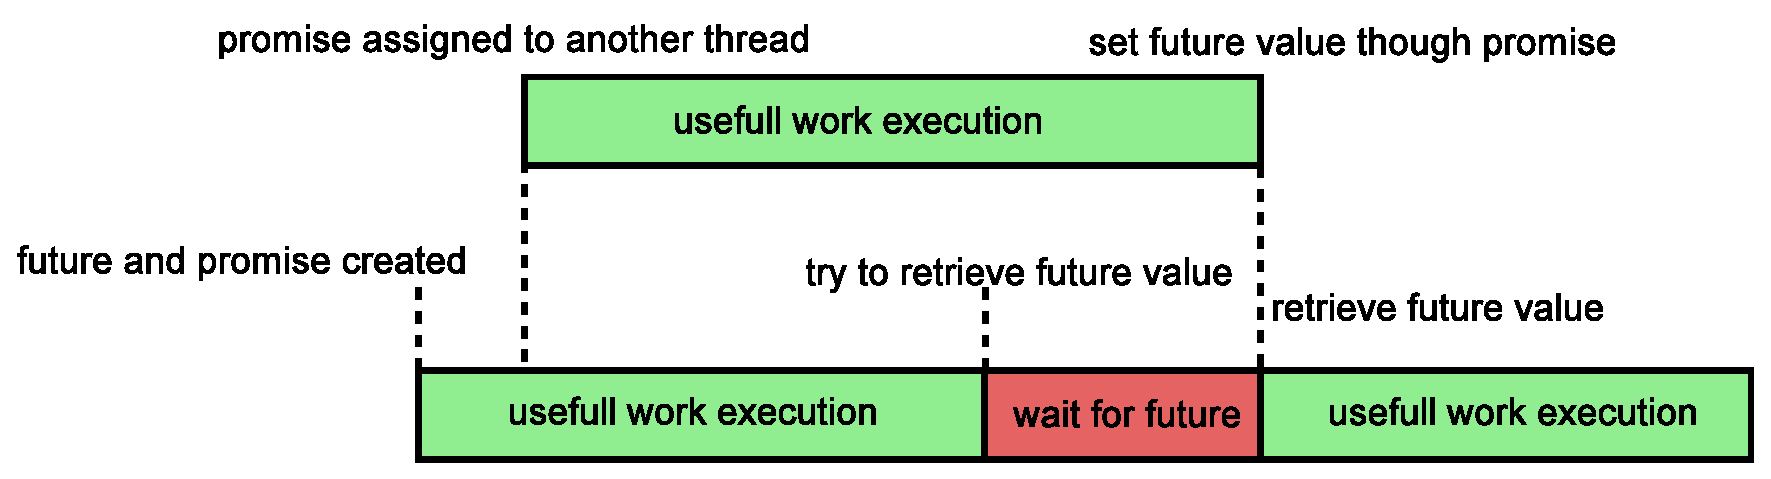
\includegraphics[width=\columnwidth]{images/futures_blocking}
\end{figure}
\end{frame}
%%%%%%%%%%%%%%%%%%%%%%%%%%%%%%%%%%%%%%%%%%%%%%%%%%%%%%%%%%%%%%%%%%%%%%%%%%%%%%%%%%%%%%%%
\defverbatim[colored]\lstFuturesBlocking{
\begin{lstlisting}
int	fibonacci(int n) {
	if(n == 0) return 0;
	if(n == 1) return 1;
	future<int> fib1 = async(fibonacci, n-1);
	future<int> fib2 = async(fibonacci, n-2);
	return fib1.get() + fib2.get();
}
\end{lstlisting}
}
\begin{frame}[fragile]{C++ Futures Interface:Fibonacci}
\note[item]{In the scope of this work, we care about the C++ futures interface}
\note[item]{Well integrated in generic programming.}
\note[item]{Describe flow of example}
\note[item]{Very easy to use.  Very close to sequential code}
\lstFuturesBlocking
\end{frame}
%%%%%%%%%%%%%%%%%%%%%%%%%%%%%%%%%%%%%%%%%%%%%%%%%%%%%%%%%%%%%%%%%%%%%%%%%%%%%%%%%%%%%%%%
\subsection{Asynchronous Communication}
\begin{frame}{Asynchronous Communication}
\note[item]{We talked about asynchronous execution, but what about communication}
\begin{itemize}
	\item PGAS and RPC both require asynchronous communication
	\item Futures is an asynchronous execution model
	\begin{itemize}
		\item In Shared Memory easy to implement
		\note[item]{Data is shared, future reads data, promise sets it}
		\item<2-> \textcolor{red}{What about Distributed Memory?}
		\item<3-> Answer:Asynchronous communication
	\end{itemize}
\end{itemize}
\end{frame}
%%%%%%%%%%%%%%%%%%%%%%%%%%%%%%%%%%%%%%%%%%%%%%%%%%%%%%%%%%%%%%%%%%%%%%%%%%%%%%%%%%%%%%%%
\begin{frame}{Asynchronous Communication}
\begin{itemize}
	\item Emulate asynchrony
	\note[item]{Number of Ways to emulate asynchronous communication}
	\begin{itemize}
		\item Polling for messages
		\note[item]{Worker polls for messages at a predefined time iterval}
		\begin{itemize}
			\item Unresponsive it time interval is small
			\item Polling can dominate computation if time interval too great
		\end{itemize}
		\item Hardware Interrupts
		\begin{itemize}
			\item High cost
			\note[item]{usually interupts need to go through the OS, very expensive}
			\item Not always available
		\end{itemize}
		\item Dedicating a thread for communication
			\note[item]{probing for messages or blocking}
		\begin{itemize}
			\item Performance depends on thread implementation and OS
		\end{itemize}
	\end{itemize}
	\item<2-> One-sided communication (MPI-2, ARMCI)
	\note[item]{we are insterested in MPI-2, highly available, de-facto in distributed machines.  Infamous one-sided interface}
\end{itemize}
\end{frame}
%%%%%%%%%%%%%%%%%%%%%%%%%%%%%%%%%%%%%%%%%%%%%%%%%%%%%%%%%%%%%%%%%%%%%%%%%%%%%%%%%%%%%%%%
\subsection{MPI-2 One-sided Communication}
\begin{frame}{MPI-2 One-sided Communication}
\begin{adjustbox}{max totalsize={.9\textwidth}{.7\textheight},center}
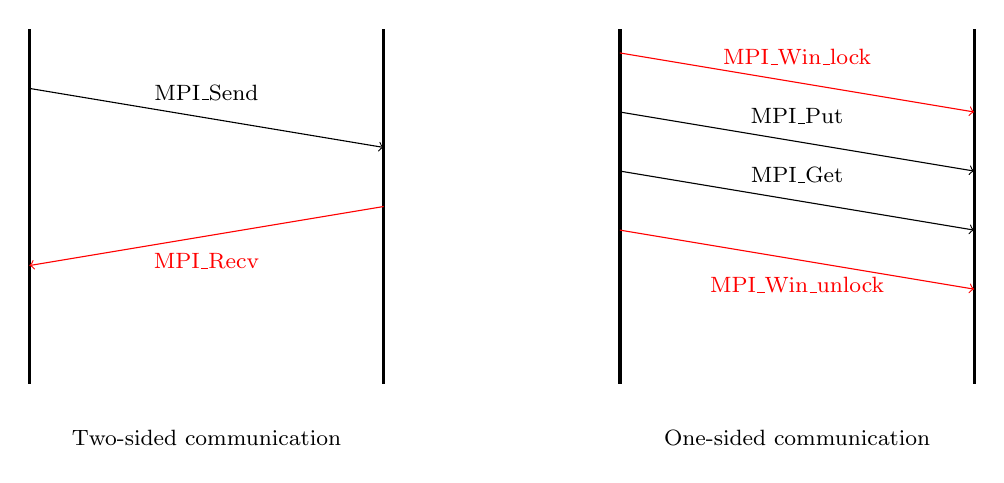
\begin{tikzpicture}[node distance = 1cm, scale=1.5, font=\footnotesize,
end/.style={very thick}]
	%comm ends
  \draw[end] (0,0) -- (0, 3);
	\draw[end] (3,0) -- (3, 3);
	%comm actions
  \draw[->] (0,2.5) -> (3, 2) node[pos=0.5, above=0.1] {MPI\_Send};
  \draw[->, color=red] (3,1.5) -> (0, 1) node[pos=0.5, below=0.1] (mpiRecv) {MPI\_Recv};

	\node[below=1.8 of mpiRecv] {Two-sided communication};

	%comm ends
  \draw[end] (5,0) -- (5, 3);
	\draw[end] (8,0) -- (8, 3);
	%comm actions
  \draw[->, color=red] (5,2.8) -> (8, 2.3) node[pos=0.5, above=0.1] {MPI\_Win\_lock};
  \draw[->] (5,2.3) -> (8, 1.8) node[pos=0.5, above=0.1] {MPI\_Put};
  \draw[->] (5,1.8) -> (8, 1.3) node[pos=0.5, above=0.1] {MPI\_Get};
  \draw[->, color=red] (5,1.3) -> (8, 0.8) node[pos=0.5, below=0.1] (winUnlock) {MPI\_Win\_unlock};

	\node[below=1.5 of winUnlock] {One-sided communication};
	
\end{tikzpicture}
\end{adjustbox}
\end{frame}
%%%%%%%%%%%%%%%%%%%%%%%%%%%%%%%%%%%%%%%%%%%%%%%%%%%%%%%%%%%%%%%%%%%%%%%%%%%%%%%%%%%%%%%%
\begin{frame}{MPI-2 One-sided Communication}
\begin{adjustbox}{max totalsize={.9\textwidth}{.7\textheight},center}
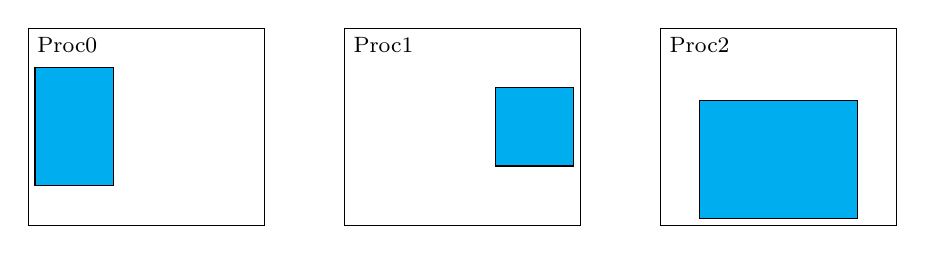
\begin{tikzpicture}[node distance = 1cm, scale=1.5, font=\footnotesize,
proc_mem/.style={draw, rectangle, minimum width=3cm, minimum height=2.5cm},
shared_mem/.style={draw, rectangle, fill=cyan}]
	%process memory
	\node[proc_mem] (Proc0) {};
	\node[anchor=north west] at (Proc0.north west) {Proc0};
	\node[proc_mem, right=1cm of Proc0] (Proc1) {};
	\node[anchor=north west] at (Proc1.north west) {Proc1};
	\node[proc_mem, right=1cm of Proc1] (Proc2) {};
	\node[anchor=north west] at (Proc2.north west) {Proc2};

	%shared windows
	\node[shared_mem, minimum width=1cm, minimum height=1.5cm, left=-1.1cm of Proc0] {};
	\node[shared_mem, minimum width=1cm, minimum height=1cm, right=-1.1cm of Proc1] {};
	\node[shared_mem, minimum width=2cm, minimum height=1.5cm, below=-1.6cm of Proc2] {};
	
\end{tikzpicture}
\end{adjustbox}
\begin{itemize}
	\item Local data is exposed through \texttt{MPI\_Window} objects
	\item Windows are created by calling the \texttt{MPI\_Win\_create}
	\note[item]{Windows can be of different size, on each process, even null}
	\note[item]{Referencing data on a window is done by providing the process id and displacement from starting pointer address}
	\item \texttt{MPI\_Win\_create} is a collective operation
	\item All dymacially allocated data shared by a window must be allocated with \texttt{MPI\_Alloc\_mem}
\end{itemize}
\end{frame}
%%%%%%%%%%%%%%%%%%%%%%%%%%%%%%%%%%%%%%%%%%%%%%%%%%%%%%%%%%%%%%%%%%%%%%%%%%%%%%%%%%%%%%%%
\begin{frame}{MPI-2 One-sided Communication}
\begin{adjustbox}{max totalsize={.9\textwidth}{.7\textheight},center}
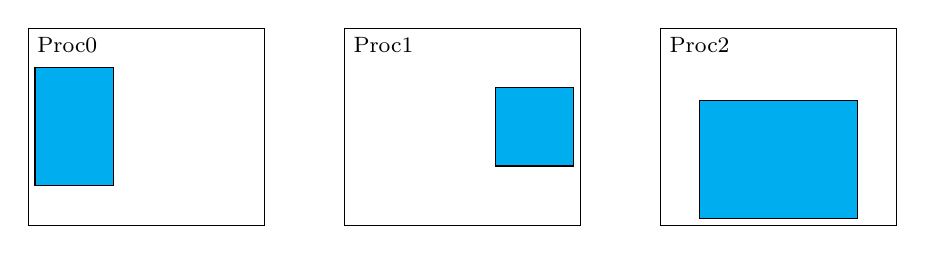
\begin{tikzpicture}[node distance = 1cm, scale=1.5, font=\footnotesize,
proc_mem/.style={draw, rectangle, minimum width=3cm, minimum height=2.5cm},
shared_mem/.style={draw, rectangle, fill=cyan}]
	%process memory
	\node[proc_mem] (Proc0) {};
	\node[anchor=north west] at (Proc0.north west) {Proc0};
	\node[proc_mem, right=1cm of Proc0] (Proc1) {};
	\node[anchor=north west] at (Proc1.north west) {Proc1};
	\node[proc_mem, right=1cm of Proc1] (Proc2) {};
	\node[anchor=north west] at (Proc2.north west) {Proc2};

	%shared windows
	\node[shared_mem, minimum width=1cm, minimum height=1.5cm, left=-1.1cm of Proc0] {};
	\node[shared_mem, minimum width=1cm, minimum height=1cm, right=-1.1cm of Proc1] {};
	\node[shared_mem, minimum width=2cm, minimum height=1.5cm, below=-1.6cm of Proc2] {};
\end{tikzpicture}
\end{adjustbox}
\begin{itemize}
	\item Remote put/get operations can be performed on memory windows
	\note[item]{These are equivalent to send/receive calls, but need not be paired}
	\item These operations must happen in an "epoch"
	\item An "epoch" is a time frame defined by successive calls of the MPI synchronization primitives \\
				\textcolor{blue}{More on that Later!} 
\end{itemize}
\end{frame}
%%%%%%%%%%%%%%%%%%%%%%%%%%%%%%%%%%%%%%%%%%%%%%%%%%%%%%%%%%%%%%%%%%%%%%%%%%%%%%%%%%%%%%%%
\defverbatim[colored]\lstMPIPut{
\begin{lstlisting}
$\tikzmark{MPIPut}$MPI_Put(base_ptr, size, datatype, 1, offset,
    		size, datatype, window);
\end{lstlisting}
}

\begin{frame}{MPI-2 One-sided Communication}
\begin{adjustbox}{max totalsize={.9\textwidth}{.7\textheight},center}
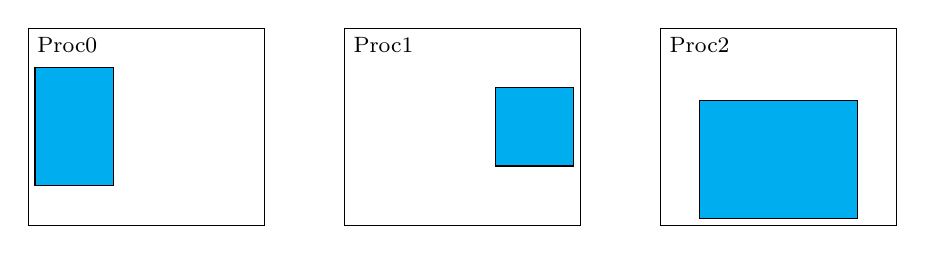
\begin{tikzpicture}[node distance = 1cm, scale=1.5, font=\footnotesize, remember picture,
proc_mem/.style={draw, rectangle, minimum width=3cm, minimum height=2.5cm},
shared_mem/.style={draw, rectangle, fill=cyan}]
	%process memory
	\node[proc_mem] (Proc0) {};
	\node[anchor=north west] at (Proc0.north west) {Proc0};
	\node[proc_mem, right=1cm of Proc0] (Proc1) {};
	\node[anchor=north west] at (Proc1.north west) {Proc1};
	\node[proc_mem, right=1cm of Proc1] (Proc2) {};
	\node[anchor=north west] at (Proc2.north west) {Proc2};

	%shared windows
	\node[shared_mem, minimum width=1cm, minimum height=1.5cm, left=-1.1cm of Proc0] {};
	\node[shared_mem, minimum width=1cm, minimum height=1cm, right=-1.1cm of Proc1] {};
	\node[shared_mem, minimum width=2cm, minimum height=1.5cm, below=-1.6cm of Proc2] {};
\end{tikzpicture}
\end{adjustbox}
\vfill

\lstMPIPut
\tikz[overlay,remember picture] \draw[->, color=red] ($(MPIPut)+(1, 0.3)$) -- ($(Proc1)$);

\note[item]{base\_ptr is the base pointer of the buffer that contains the data to be send}
\note[item]{size is the number of elements the buffer contains and the number of elements 
			to be read from the remot location}
\note[item]{id is the rank of the process}
\note[item]{offset is the offset from the start of the windows on process with rank id}
\note[item]{window is the \texttt{MPI\_Window} that the operation will be applied on}
\end{frame}
%%%%%%%%%%%%%%%%%%%%%%%%%%%%%%%%%%%%%%%%%%%%%%%%%%%%%%%%%%%%%%%%%%%%%%%%%%%%%%%%%%%%%%%%
\defverbatim[colored]\lstMPIGet{
\begin{lstlisting}
$\tikzmark{MPIGet}$MPI_Get(base_ptr, size, datatype, 2, offset,
    		size, datatype, window);
\end{lstlisting}
}

\begin{frame}{MPI-2 One-sided Communication}
\begin{adjustbox}{max totalsize={.9\textwidth}{.7\textheight},center}
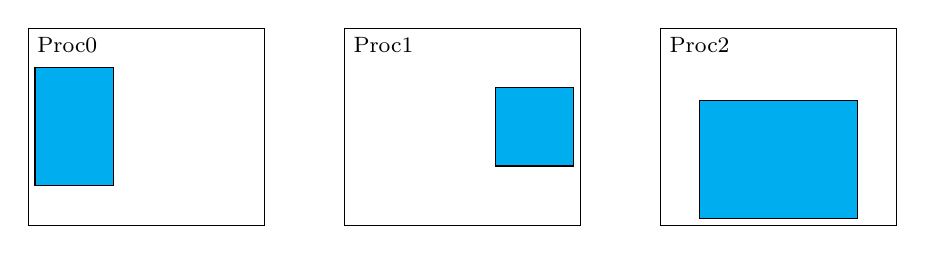
\begin{tikzpicture}[node distance = 1cm, scale=1.5, font=\footnotesize, remember picture,
proc_mem/.style={draw, rectangle, minimum width=3cm, minimum height=2.5cm},
shared_mem/.style={draw, rectangle, fill=cyan}]
	%process memory
	\node[proc_mem] (Proc0) {};
	\node[anchor=north west] at (Proc0.north west) {Proc0};
	\node[proc_mem, right=1cm of Proc0] (Proc1) {};
	\node[anchor=north west] at (Proc1.north west) {Proc1};
	\node[proc_mem, right=1cm of Proc1] (Proc2) {};
	\node[anchor=north west] at (Proc2.north west) {Proc2};

	%shared windows
	\node[shared_mem, minimum width=1cm, minimum height=1.5cm, left=-1.1cm of Proc0] {};
	\node[shared_mem, minimum width=1cm, minimum height=1cm, right=-1.1cm of Proc1] {};
	\node[shared_mem, minimum width=2cm, minimum height=1.5cm, below=-1.6cm of Proc2] {};
\end{tikzpicture}
\end{adjustbox}
\vfill

\lstMPIGet
\tikz[overlay,remember picture] \draw[->, color=red] ($(Proc2)+(-1.5,0)$) -- ($(MPIGet)+(1, 0.3)$);

\note[item]{base\_ptr is the base pointer of the buffer that contains the data to be send}
\note[item]{size is the number of elements the buffer contains and the number of elements 
			to be read from the remot location}
\note[item]{id is the rank of the process}
\note[item]{offset is the offset from the start of the windows on process with rank id}
\note[item]{window is the \texttt{MPI\_Window} that the operation will be applied on}
\end{frame}
%%%%%%%%%%%%%%%%%%%%%%%%%%%%%%%%%%%%%%%%%%%%%%%%%%%%%%%%%%%%%%%%%%%%%%%%%%%%%%%%%%%%%%%%
\begin{frame}{MPI-2 One-sided Communication}
	\begin{itemize}
		\item Put and Get operations need to be synchronized!\\
					\textcolor{blue}{Remember "epochs"}?
		\note[item]{As in shared memory, put and get have to be synchronized}
		\item Why?
		\begin{itemize}
			\item Concurrent accesses to the same window and overlapping data are erroneus
			\item End of "epoch" marks that message was send or received
			\note[item]{Necessary for synchronization of messages - still a message passing library} 
		\end{itemize}
		\item Two modes of synchronization
		\begin{itemize}
			\item Active mode: All processes are required to take part in the synchronization
			\item Passive mode: Only the process initiating the put/get operation needs to synchronize
		\end{itemize}
	\end{itemize}
\end{frame}
%%%%%%%%%%%%%%%%%%%%%%%%%%%%%%%%%%%%%%%%%%%%%%%%%%%%%%%%%%%%%%%%%%%%%%%%%%%%%%%%%%%%%%%%
\begin{frame}{MPI-2 One-sided Communication}
\begin{adjustbox}{max totalsize={.9\textwidth}{.7\textheight},center}
\begin{tikzpicture}[node distance = 1cm, scale=1.5, font=\footnotesize,
end/.style={very thick}]
	%comm ends
  \draw[end] (0,0) -- (0, 3);
	\draw[end] (3,0) -- (3, 3);
	%comm actions
  \draw[dashed, color=red] (0,2.5) -> (3, 2.5) node[pos=0.5, above=0.1] (startEpoch) {};
  \draw[->] (0,2.3) -> (3, 1.8) node[pos=0.5, above=0.1] {MPI\_Put};
  \draw[->] (0,1.8) -> (3, 1.3) node[pos=0.5, above=0.1] {MPI\_Get};
  \draw[dashed, color=red] (0,1) -> (3, 1) node[pos=0.5, below=0.1] (endEpoch) {};

	\node[color=red] at (-0.8,2.5) {MPI\_Win\_start};
	\node[color=red] at (-1,1) {MPI\_Win\_complete};
	\node[color=red] at (3.8,2.5) {MPI\_Win\_post};
	\node[color=red] at (3.8,1) {MPI\_Win\_wait};

	\node[below=1.8 of mpiRecv] {Active Mode};

	%comm ends
  \draw[end] (6.3,0) -- (6.3, 3);
	\draw[end] (9.3,0) -- (9.3, 3);
	%comm actions
  \draw[dashed, color=red] (6.3,2.5) -> (9.3, 2.5) node[pos=0.5, above=0.1] {};
  \draw[->] (6.3,2.3) -> (9.3, 1.8) node[pos=0.5, above=0.1] {MPI\_Put};
  \draw[->] (6.3,1.8) -> (9.3, 1.3) node[pos=0.5, above=0.1] {MPI\_Get};
  \draw[dashed, color=red] (6.3,1) -> (9.3, 1) node[pos=0.5, below=0.1] (winUnlock) {};

	\node[color=red] at (5.5,2.5) {MPI\_Win\_fence};
	\node[color=red] at (5.5,1) {MPI\_Win\_fence};
	\node[color=red] at (10.1,2.5) {MPI\_Win\_fence};
	\node[color=red] at (10.1,1) {MPI\_Win\_fence};

	\node[below=1.5 of winUnlock] {Active Mode/Collective};
	
\end{tikzpicture}
\end{adjustbox}
\begin{itemize}
	\item All processes must be aware of the other processes that take part in the communication
	\note[item]{know each other's rank or be in the group}
	\item Communication is \textcolor{red}{not} initiated \textcolor{red}{asynchronously}
	\note[item]{does not fit our purpose, would require again polling etc. Only completion is asynchronous}
\end{itemize}
\end{frame}
%%%%%%%%%%%%%%%%%%%%%%%%%%%%%%%%%%%%%%%%%%%%%%%%%%%%%%%%%%%%%%%%%%%%%%%%%%%%%%%%%%%%%%%%
\begin{frame}{MPI-2 One-sided Communication}
\begin{adjustbox}{max totalsize={.4\textwidth}{.4\textheight},center}
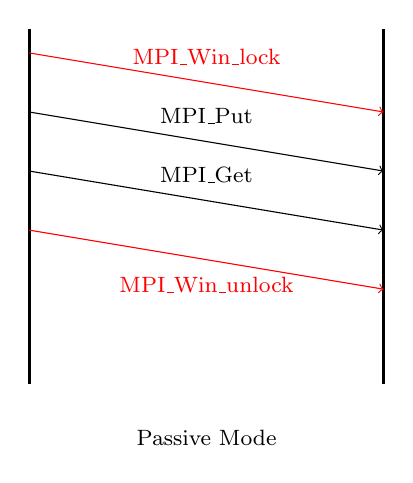
\begin{tikzpicture}[node distance = 1cm, scale=1.5, font=\footnotesize,
end/.style={very thick}]
	%comm ends
  \draw[end] (5,0) -- (5, 3);
	\draw[end] (8,0) -- (8, 3);
	%comm actions
  \draw[->, color=red] (5,2.8) -> (8, 2.3) node[pos=0.5, above=0.1] {MPI\_Win\_lock};
  \draw[->] (5,2.3) -> (8, 1.8) node[pos=0.5, above=0.1] {MPI\_Put};
  \draw[->] (5,1.8) -> (8, 1.3) node[pos=0.5, above=0.1] {MPI\_Get};
  \draw[->, color=red] (5,1.3) -> (8, 0.8) node[pos=0.5, below=0.1] (winUnlock) {MPI\_Win\_unlock};

	\node[below=1.5 of winUnlock] {Passive Mode};
	
\end{tikzpicture}
\end{adjustbox}
\begin{itemize}
	\item Really asynchronous!
	\note[item]{Other process need not take any action}
	\item Can only write/read data allocated with \texttt{MPI\_Alloc\_mem}
	\item \texttt{MPI\_Win\_lock} can only be acquired for the whole window
	\note[item]{even non-overlapping accesses must me protected}
	\item Not real locks, cannot be used to define critical regions
\end{itemize}
\end{frame}
%%%%%%%%%%%%%%%%%%%%%%%%%%%%%%%%%%%%%%%%%%%%%%%%%%%%%%%%%%%%%%%%%%%%%%%%%%%%%%%%%%%%%%%%
\section{MPI Futures}
\subsection{Overview}
\begin{frame}{MPI Futures}
\begin{itemize}
	\item C++11 standard library future interface over message passing
	\item Modular design
	\note[item]{each module implementation is transparent to the others.  Only need to provide the API interface functionality}
	\begin{itemize}
		\item Scheduler:
			\begin{itemize}
				\item Distributes asynchronous functions (aka \emph{jobs})
				\item Maintains stacks to keep \emph{jobs}, on each process
			\end{itemize}
		\item Shared Memory Manager:
			\begin{itemize}
				\item Provides a virtual shared memory view  through a \texttt{Shared\_ptr} variable
				\item Provides the routines to read/write and allocate data on the virtual shared address space 
				\note[item]{memory could be distributed in truth} 
			\end{itemize}
		\item Communication Manager:
			\begin{itemize}
				\item Provides asynchronous message passing
				\item Provides a mechanism to expose share local process space
				\item Implemented using MPI one-sided communication library
			\end{itemize}
	\end{itemize}
\end{itemize}	 
\end{frame}
%%%%%%%%%%%%%%%%%%%%%%%%%%%%%%%%%%%%%%%%%%%%%%%%%%%%%%%%%%%%%%%%%%%%%%%%%%%%%%%%%%%%%%%%
\subsection{Interface}
\defverbatim[colored]\lstFibMPI{
\begin{adjustbox}{max totalsize={.5\textwidth}}
\begin{lstlisting}
class fib {
public:
	fib() {};
	~fib() {};
	int	operator()(int n) {
		if(n == 0) return 0;
		if(n == 1) return 1;
		fib f;
		future<int> fib1 = async(f, n-1);
		future<int> fib2 = async(f, n-2);
		return fib1.get() + fib2.get();;
	};
};

FUTURES_SERIALIZE_CLASS(fib);
FUTURES_EXPORT_FUNCTOR((async_function<fib, int>));

\end{lstlisting}
\end{adjustbox}
}
\begin{frame}[fragile]{MPI Futures:Interface}
\lstFibMPI
\note[item]{Very important EXPORT_FUNCTOR. Exposes function to MPI and serialization}
\begin{itemize}
	\item Only functor objects can be issued with an \texttt{async}
	\item Functor and its arguments must be serializable
\end{itemize}	 
\end{frame}
%%%%%%%%%%%%%%%%%%%%%%%%%%%%%%%%%%%%%%%%%%%%%%%%%%%%%%%%%%%%%%%%%%%%%%%%%%%%%%%%%%%%%%%%
\begin{frame}[fragile]{MPI Futures:Interface}
\begin{itemize}
	\item If return value size can change dynamically (pointer, vectors, etc) the size must be provided to \texttt{async}
	\item User can call \texttt{async\_on} and provide the rank of the process he wants it scheduled on
	\note[item]{Skips scheduler.  Can take advantage of data locality} 
	\begin{itemize}
		\item Take advantage of how data locality
		\item More effective data and work distribution
		\note[item]{Remember, data is also distributed with an async call} 
	\end{itemize}
\end{itemize}	 
\end{frame}
%%%%%%%%%%%%%%%%%%%%%%%%%%%%%%%%%%%%%%%%%%%%%%%%%%%%%%%%%%%%%%%%%%%%%%%%%%%%%%%%%%%%%%%%
\subsection{Implementation}
\begin{frame}{MPI Futures:Implementation}
\begin{adjustbox}{max totalsize={.9\textwidth}{.7\textheight},center}
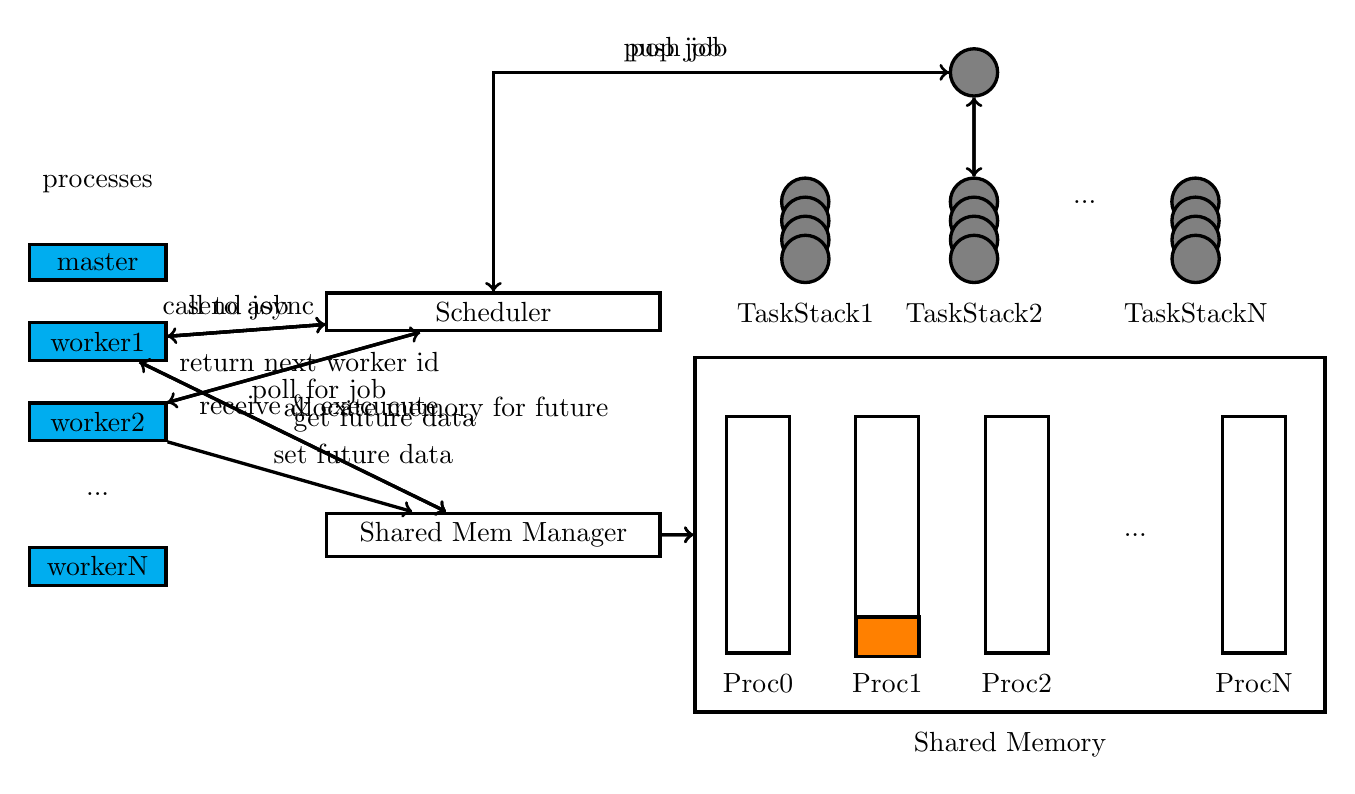
\begin{tikzpicture}[very thick, node distance = 1cm, scale=0.1,
% STYLES
every node/.style={text badly centered},
tq/.style={draw, circle, minimum width=0.6cm, fill=gray},
txt/.style={text badly centered},
proc/.style={draw, rectangle, text badly centered, text width=1.5cm, fill=cyan},
mem_node/.style={draw, rectangle, minimum height=3cm, minimum width=0.8cm}]
	%processes nodes
  \node[proc] (proc0) {master};
	\node[proc, below=0.5cm of proc0] (proc1) {worker1};
	\node[proc, below=0.5cm of proc1] (proc2) {worker2};
	\node[rectangle, below=0.5cm of proc2] (proc_space) {...};
	\node[proc, below=0.5cm of proc_space] (procN) {workerN};
	\node[above=0.5 of proc0] {processes};
	%modules nodes
	\node[rectangle, right=4cm of proc2] (modules_anchor) {};
  \node[draw, rectangle, text width=4cm, above=1cm of modules_anchor] (sched) {Scheduler};
	\node[draw, rectangle, text width=4cm, below=1cm of modules_anchor] (shmem) {Shared Mem Manager};
	%dummy node to help alignment
	\node[rectangle, above=1cm of sched] (sched_aux) {}; 
	%task stacks nodes
	\node[tq, right=3.5cm of sched_aux] (tq1_head) {};
	\node[tq, below=-0.4cm of tq1_head] (tq1_n1) {};
	\node[tq, below=-0.4cm of tq1_n1] (tq1_n2) {};
	\node[tq, below=-0.4cm of tq1_n2] (tq1_n3) {};

	\node[tq, right=1.5cm of tq1_head] (tq2_head) {};
	\node[tq, below=-0.4cm of tq2_head] (tq2_n1) {};
	\node[tq, below=-0.4cm of tq2_n1] (tq2_n2) {};
	\node[tq, below=-0.4cm of tq2_n2] (tq2_n3) {};

	\node[rectangle, right=0.8cm of tq2_head] (tq_space) {...};

	\node[tq, right=0.8cm of tq_space] (tqN_head) {};
	\node[tq, below=-0.4cm of tqN_head] (tqN_n1) {};
	\node[tq, below=-0.4cm of tqN_n1] (tqN_n2) {};
	\node[tq, below=-0.4cm of tqN_n2] (tqN_n3) {};

	\node[txt, rectangle, below=0.1cm of tq1_n3] {TaskStack1};
	\node[txt, rectangle, below=0.1cm of tq2_n3] {TaskStack2};
	\node[txt, rectangle, below=0.1cm of tqN_n3] {TaskStackN};

	%process sharem memory nodes
	\node[draw, rectangle, minimum height=4.5cm, minimum width=8cm, right=0.4 of shmem] (shmem_box) {};
	\node[txt, rectangle, below=0.1cm of shmem_box] {Shared Memory};

	\node[mem_node, right=0.8 of shmem] (mn0) {};
	\node[mem_node, right=0.8 of mn0] (mn1) {};
	\node[mem_node, right=0.8 of mn1] (mn2) {};
	\node[rectangle, right=0.8cm of mn2] (mn_space) {...};
	\node[mem_node, right=0.8 of mn_space] (mnN) {};

	\node[txt, rectangle, below=0.1cm of mn0] {Proc0};
	\node[txt, rectangle, below=0.1cm of mn1] {Proc1};
	\node[txt, rectangle, below=0.1cm of mn2] {Proc2};
	\node[txt, rectangle, below=0.1cm of mnN] {ProcN};


  % 1st pass: draw arrows
  \onslide<2>\draw[->] (proc1) -> (sched) node[pos=0.45, above] {call to async};
	\onslide<3>\draw[->] (sched) -> (proc1) node[pos=0.1, below=0.2cm] {return next worker id};
	\onslide<4>\draw[->] (proc1) -> (shmem) node[pos=1, above=1] {allocate memory for future};
	\onslide<4>\draw[->] (shmem) -> (shmem_box) node[pos=0.1, below=0.2cm] {};
	\onslide<4-7>\node[draw, rectangle, below=-0.5cm of mn1, minimum height=0.5cm, minimum width=0.8cm, fill=gray] {};
	\onslide<5>\draw[->] (proc1) -> (sched) node[pos=0.45, above] {send job};
	\onslide<5,7>\node[tq, above=1cm of tq2_head] (new_job) {};
	\onslide<5>\draw[->] (sched) |- (new_job) node[pos=0.7, above] {push job};
	\onslide<5>\draw[->] (new_job) -> (tq2_head);
	\onslide<6>\draw[->] (proc2) -> (sched) node[pos=0.6, below=0.1cm] {poll for job};
	\onslide<7>\draw[->] (sched) -> (proc2) node[pos=0.4, below=0.3cm] {receive \& execucute};
	\onslide<7>\draw[->] (new_job) -| (sched) node[pos=0.3, above] {pop job};
	\onslide<7>\draw[->] (tq2_head) -> (new_job);
	\onslide<8>\draw[->] (proc2) -> (shmem) node[pos=0.8, above=0.3] {set future data};
	\onslide<8->\draw[->] (shmem) -> (shmem_box) node[pos=0.1, below=0.2cm] {};
	\onslide<8->\node[draw, rectangle, below=-0.5cm of mn1, minimum height=0.5cm, minimum width=0.8cm, fill=orange] {};
	\onslide<9>\draw[<->] (proc1) -> (shmem) node[pos=0.8, above=0.5] {get future data};
\end{tikzpicture}
\end{adjustbox}
\end{frame}
%%%%%%%%%%%%%%%%%%%%%%%%%%%%%%%%%%%%%%%%%%%%%%%%%%%%%%%%%%%%%%%%%%%%%%%%%%%%%%%%%%%%%%%%
\section{Evaluation}
\subsection{Interface Assesment}

\defverbatim[colored]\lstFutCompare{
\begin{adjustbox}{max totalsize={.8\textwidth}}
\begin{minipage}{.48\textwidth}
\begin{lstlisting}
class fib {
public:
	fib() {};
	~fib() {};
	int	operator()(int n) {
		if(n == 0) return 0;
		if(n == 1) return 1;
		fib f;
		future<int> fib1 = async(f, n-1);
		future<int> fib2 = async(f, n-2);
		return fib1.get() + fib2.get();;
	};
};

FUTURES_SERIALIZE_CLASS(fib);
FUTURES_EXPORT_FUNCTOR((async_function<fib, int>));
\end{lstlisting}
\end{minipage}
\hspace{4cm}
\begin{minipage}{.48\textwidth}
\begin{lstlisting}
int	fibonacci(int n) {
	if(n == 0) return 0;
	if(n == 1) return 1;
	future<int> fib1 = async(fibonacci, n-1);
	future<int> fib2 = async(fibonacci, n-2);
	return fib1.get() + fib2.get();
}
\end{lstlisting}
\end{minipage}
\end{adjustbox}
}
\begin{frame}[fragile]{Interface Assesment}
\lstFutCompare
\begin{itemize}
	\item Very close to the C++11 standard!
	\item Easy to use compared to original message passing code
	\item Easy to expose functor objects to worker processes
\end{itemize}
\end{frame}
%%%%%%%%%%%%%%%%%%%%%%%%%%%%%%%%%%%%%%%%%%%%%%%%%%%%%%%%%%%%%%%%%%%%%%%%%%%%%%%%%%%%%%%%
\section{Evaluation}
\subsection{Interface Assesment}
\begin{frame}{Interface Assesment}
Limitations
\begin{itemize}
		\item Only serializable functor objects can be issued by
		\item Arguments must also be serializable
		\note[item]{also additional overhead}
		\item Size of dynamically sized objects as return values must be declared at \emph{async} callsite 
\end{itemize}
\end{frame}
%%%%%%%%%%%%%%%%%%%%%%%%%%%%%%%%%%%%%%%%%%%%%%%%%%%%%%%%%%%%%%%%%%%%%%%%%%%%%%%%%%%%%%%%
\subsection{Performance}
\begin{frame}{Performance Evaluation:Setup}
Evaluation setup:
\begin{itemize}
	\item 2 Intel(R) Xeon(R) CPU E5645@2.40 GHz with 6 available cores on each machine
	\item Connected through a network socket, but provide shared space interface
	\item Compiled using g++ version 4.6.3 with level 3 optimization enabled
	\item OpenMPI version 1.4.3
	\item Boost serialization version ??
\end{itemize}
\end{frame}
%%%%%%%%%%%%%%%%%%%%%%%%%%%%%%%%%%%%%%%%%%%%%%%%%%%%%%%%%%%%%%%%%%%%%%%%%%%%%%%%%%%%%%%%
\begin{frame}{Performance Evaluation:Benchmarks}
Three benchmarks:
\vfill
\begin{itemize}
	\item Fibonacci:
	\begin{itemize}
		\item We run it for a == 45
		\item For a $<$ 30, we run the sequential code
		\note[item]{Need to have some work done, 30 is pretty fast}
	\end{itemize} 
\vfill
	\item Quicksort:
	\begin{itemize}
		\item We run it for sorting 100,000 elements
		\item For n $<$ ??, we run the sequential code
		\note[item]{after every return of async, we need to merge the two arrays, lots of copies}
	\end{itemize}
\vfill
	\item Tiled LU
	\begin{itemize}
		\item<2-> \textcolor{red}{A little more complicated...}
	\end{itemize} 
\end{itemize}
\end{frame}
%%%%%%%%%%%%%%%%%%%%%%%%%%%%%%%%%%%%%%%%%%%%%%%%%%%%%%%%%%%%%%%%%%%%%%%%%%%%%%%%%%%%%%%%
\defverbatim[colored]\lstTLU{
\begin{adjustbox}{max totalsize={0.8\textwidth}}
\begin{minipage}{.45\textwidth}
\begin{lstlisting}
for(int k = 0; k < TOTAL_TILES; k++) {
	dgetrf(A[k][k], P[k][k]);
	for(int n = k+1; n < TOTAL_TILES; n++) {
		dgessm(A[k][n], A[k][k], P[k][k])
	}
  for(int m = k+1; m < TOTAL_TILES; m++) {
		dtstrf(A[k][k], A[m][k] , P[m][k]);
  	for(int n=k+1; n < TOTAL_TILES; n++) {
			dssssm(U[k][n], A[m][n], L[m][k], 
											A[m][k], P[m][k]);
		}
	}
}
\end{lstlisting}
\end{minipage}
\hspace{4cm}
\begin{minipage}{.45\textwidth}
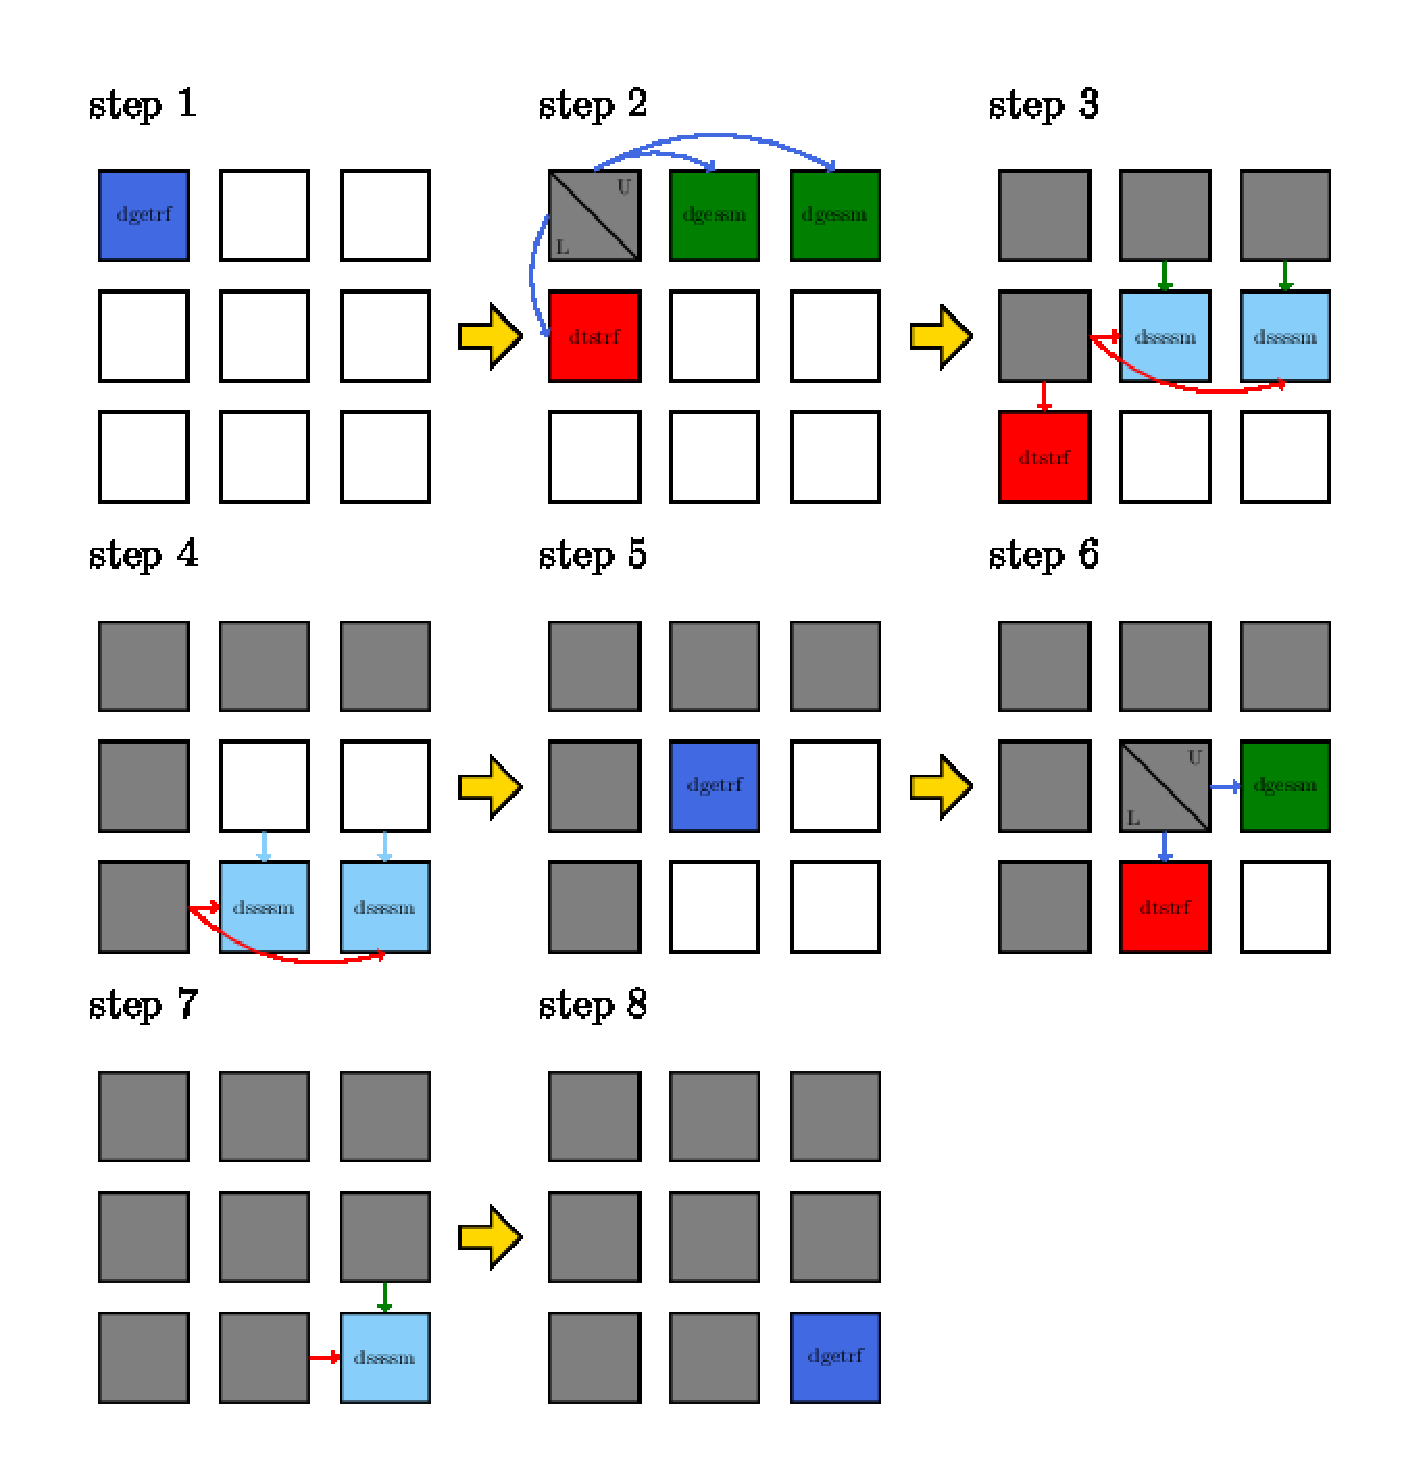
\includegraphics[width=1.5\textwidth]{images/3x3example}
\end{minipage}
\end{adjustbox}
}
\begin{frame}[fragile]{Performance Evaluation:Tiled LU}
\lstTLU
\begin{itemize}
	\item Originally implemented with PLASMA
\end{itemize}
\end{frame}
%%%%%%%%%%%%%%%%%%%%%%%%%%%%%%%%%%%%%%%%%%%%%%%%%%%%%%%%%%%%%%%%%%%%%%%%%%%%%%%%%%%%%%%%
\defverbatim[colored]\lstPTLU{
\begin{adjustbox}{max totalsize={0.8\textwidth}}
\begin{minipage}{.3\textwidth}
\begin{lstlisting}
for(int k = 0; k < TOTAL_TILES; k++) {
	A[k][k] = cpldAU[k][k].get().A;
	dgetrf(A[k][k], P[k][k]);
	for(int n = k+1; n < TOTAL_TILES; n++) {
		A[k][n] = cpldAU[k][n].get().A;
		fA[k][n] = async(dgessm, A[k][n], 
										 A[k][k], P[k][k]);
	}
  for(int m = k+1; m < TOTAL_TILES; m++) {
		A[m][k] = cpldAU.get().A;
		dtstrf(A[k][k], A[m][k].get() , P[m][k]);
  	for(int n=k+1; n < TOTAL_TILES; n++) {
			if(m == k+1)
				A[k][n] = fA[k][n].get();
			else
				A[k][n] = cpldAU.get().U;
			A[m][n] = cpldAU.get().A;
			cpldAU[m][n] = async(dssssm, A[k][n], A[m][n], 
													 L[m][k], A[m][k], P[m][k]);
		}
	}
}
\end{lstlisting}
\end{minipage}
\hspace{6cm}
\begin{minipage}{.7\textwidth}
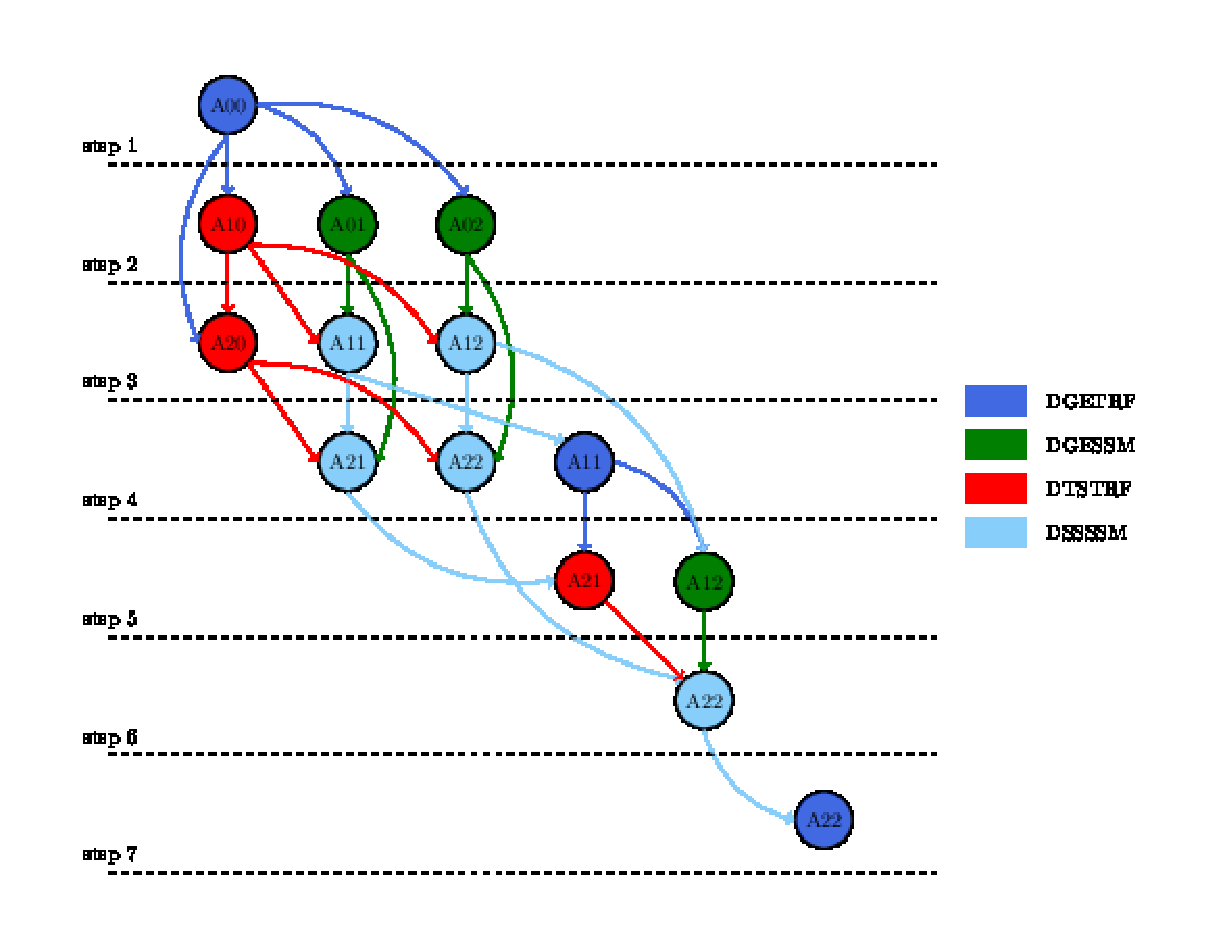
\includegraphics[width=1.5\textwidth]{images/lu_task_graph_3x3}
\end{minipage}
\end{adjustbox}
}
\begin{frame}{Performance Evaluation:Tiled LU}
\lstPTLU
\end{frame}
%%%%%%%%%%%%%%%%%%%%%%%%%%%%%%%%%%%%%%%%%%%%%%%%%%%%%%%%%%%%%%%%%%%%%%%%%%%%%%%%%%%%%%%%
\begin{frame}{Performance Evaluation}
\begin{figure}
\center
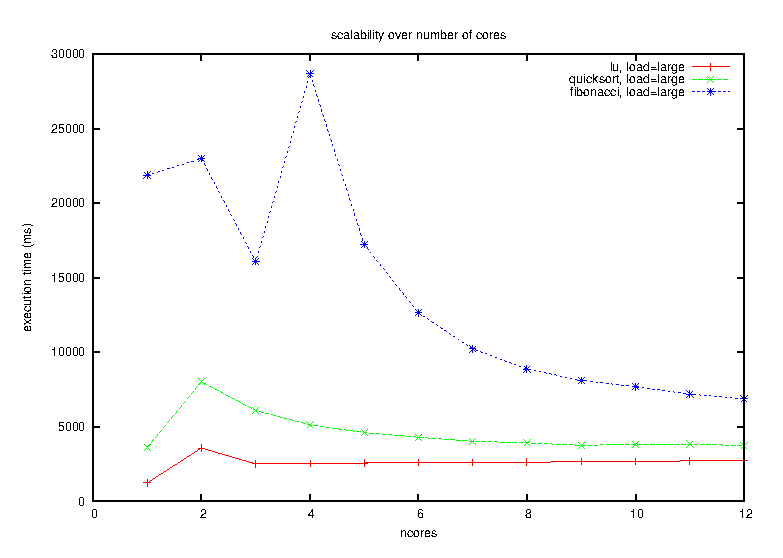
\includegraphics[width=.7\textwidth]{images/apps_scalability}
\end{figure}
\end{frame}
%%%%%%%%%%%%%%%%%%%%%%%%%%%%%%%%%%%%%%%%%%%%%%%%%%%%%%%%%%%%%%%%%%%%%%%%%%%%%%%%%%%%%%%%
\begin{frame}{Performance Evaluation}
\begin{figure}
\center
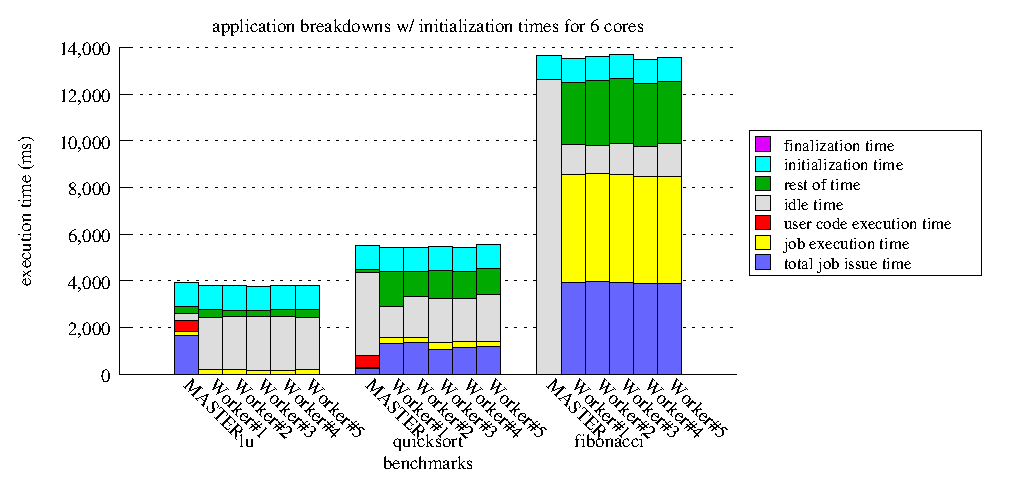
\includegraphics[width=\textwidth]{images/app_breakdowns_w_init}
\end{figure}
\end{frame}
%%%%%%%%%%%%%%%%%%%%%%%%%%%%%%%%%%%%%%%%%%%%%%%%%%%%%%%%%%%%%%%%%%%%%%%%%%%%%%%%%%%%%%%%
\begin{frame}{Conclusions}
In terms of interface we rock! Very easy to use, sensible limitations compared to shared memory
In terms of performance we suck...but we blame serialization and mpi lack of synchronization primitives
We would like these in MPI...
Maybe not completely useless?
\end{frame}
%%%%%%%%%%%%%%%%%%%%%%%%%%%%%%%%%%%%%%%%%%%%%%%%%%%%%%%%%%%%%%%%%%%%%%%%%%%%%%%%%%%%%%%%
\begin{frame}{Future Work}
Fix performance
Complete secondary feature (timeouts, exceptions, etc)
Hybrid approach, for high performance
\end{frame}
%%%%%%%%%%%%%%%%%%%%%%%%%%%%%%%%%%%%%%%%%%%%%%%%%%%%%%%%%%%%%%%%%%%%%%%%%%%%%%%%%%%%%%%%
\end{document}

